\section{PyQt}

\subsection{¿C\'omo estructurar los proyectos?}
\label{estructura_programas}
Los proyectos que involucran el dise\~no de una GUI utilizando PyQt5 estar\'an compuestos por el Backend y el Frontend, conceptos
que vienen del desarrollo web, y podes ver \href{https://platzi.com/blog/que-es-frontend-y-backend/}{ac\'a}. Entonces, tu proyecto va a tener
c\'odigo en Python de la GUI, de la l\'ogica de lo que hagas, y otros archivos como recursos, stylesheets, imagenes, etc... se propone la siguiente
estructura de archivos muy utilizada en PyQt5, y Python en algunos casos:

\begin{center}
    \begin{minipage}{10cm}
        \dirtree{%
        .1 /project.
        .2 /designer.
        .3 {mainwindow.ui}.
        .2 /resources.
        .3 {resource.qrc}.
        .3 {logo.png}.
        .2 /tests.
        .3 {test\textunderscore backend.py}.
        .2 {/src}.
        .3 {\textunderscore\textunderscore init\textunderscore \textunderscore.py}.
        .3 {app.py}.
        .3 {mainwindow.py}.
        .3 {/ui}.
        .4 {mainwindow.py}.
        .3 {/resources}.
        .4 {resources.py}.
        .2 {main.py}.
        .2 {test.py}.
        .2 requirements.
        .2 readme.
        }
    \end{minipage}
\end{center}

\subsection{¿Qu\'e son Signals, Slots?}
\label{signal_slot}

\paragraph{Signals y Slots:} Son un mecanismo de comunicaci\'on entre objetos del framework de Qt, de forma an\'aloga a c\'omo sucede en el caso de 
eventos y callbacks, en cuyo caso las Signals son los eventos y los callbacks son los Slots registrados para tales eventos.

En primer lugar, podr\'ian ya existir signals o slots dentro de una clase, o bien podr\'iamos crearlos. Usualmente sucede que cualquier m\'etodo o funci\'on dentro de Python
puede ser tomado sin problema como un Slot en el proceso de conexi\'on de dos objetos, pero no ser\'a identificado autom\'aticamente como un Slot en otros contextos.
Veamos a continuaci\'on, c\'omo podr\'iamos crear en una clase un Signal y un Slot.


\begin{lstlisting}{language=Python}
    # PyQt5 import...
    from PyQt5.QtCore import pyqtSignal
    from PyQt5.QtCore import pyqtSlot
    from PyQt5.QtCore import QObject

    # Creamos nuestra clase cualquiera, es importante que sea QObject o cualquiera
    # que haya heredado de QObject, para que pueda albergar Signals
    class MyClass(QObject):

        # Declaro de forma estatica las se\~nales de la clase
        # y como argumento de pyqtSignal se pasa el tipo de dato que
        # se manda en la comunicacion del evento, podria ser una clase
        changed = pyqtSignal()
        progress = pyqtSignal(int)

        # Creando un metodo que queremos definir como Slot,
        # tenemos que usar el decorator para poder declararlo de tal forma
        @pyqtSlot(int)
        def set_value(self, value: int):
            # Hacer algo...
            pass
\end{lstlisting}

Asumamos que ahora tenemos un objeto con eventos, luego si queremos conectar nuestro callback existen dos mecanismos. El mecanismo largo implica
que la conexi\'on est\'e declarada en t\'erminos de \textbf{ObjectoSender, Signal, Slot} y con esto se establece la conexi\'on. La forma corta implica simplemente indicarle al evento
que se le conecta un callback. A continuaci\'on un ejemplo de ambas sint\'axis.

\begin{lstlisting}{language=Python}
    """ 1era Forma """
    # Necesitamos haber realizado el import y luego la conexi\'on del
    # sender y su signal "changed" con slot llamado on_changed
    from PyQt5 import QtCore
    QtCore.QObject.connect(sender, QtCore.SIGNAL("changed()"), on_changed)

    """ 2do Forma """
    # Le indicamos al objeto y a su signal, que conecte
    # el slot para ejecutar cuando se emita el evento
    sender.changed.connect(on_changed)
\end{lstlisting}


Finalmente, asumamos que nosotros somos los que queremos notificar del evento ocurrido, si tenemos
un evento interno en nuestra clase para avisar que cambio el estado del objeto, entonces
\begin{lstlisting}{language=Python}
    # Dentro de mi clase, emito el evento "changed", que supongamos que declaramos
    # con un mensaje para aclarar o comentar cosas...
    self.changed.emit("Emitiendo este evento... llamara a todos los slots")
\end{lstlisting}

\subsection{¿Qu\'e son los Property?}
\label{qt_properties}
Cuando tenemos una clase, las variables de la instancia las solemos llamar miembros o atributos, pero en la pr\'actica se hace una diferencia
respecto de las \textbf{Propiedades}, que son variables miembro o atributos de las instancias que son accesibles \'unicamente a trav\'es de m\'etodos
Getter y Setter. Es decir, una propiedad no necesariamente es una variable, simplemente engloba los m\'etodo Getter y Setter que en su c\'odigo pueden estar
utilizando una variable miembro.

\begin{lstlisting}{language=Python}

    # Import PyQt5...
    from PyQt5.QtCore import pyqtProperty

    # Creamos los metodos para acceder internamente a las variables
    # miembro, se podria ademas ejecutar otro codigo, o hacer validacion
    # esa es la principal gracia de las Property!
    def get_name(self):
        """ Name's getter """
        return self._name
    
    def set_name(self, name: str):
        """ Name's setter """
        self._name = name

    # Habiendo creado nuestra clase... luego de forma est\'atica se crea
    # una propiedad para declararla, luego la maneja internamente para cada
    # instancia PyQt
    name = pyqtProperty(str, get_name, set_name)

\end{lstlisting}

Finalmente, trabajar externamente sobre la variable name, ser\'a de igual forma que como con una variable
interna de la clase, pero durante el get y set de tal miembro, se ejecutar\'an los m\'etodos asignados. Esto
se suele usar para \textbf{Binding}, conexi\'on entre el back-end y el front-end de una forma prolija simplemente
haciendo una conexi\'on entre una propiedad de una clase y su ViewController en la GUI.

\subsection{¿Qu\'e son los Stylesheets?}
\label{qt_stylesheets}
Los \textbf{Stylesheets} b\'asicamente es una sint\'axis que se emplea para describir el contenido de las propiedades
de un Widget que definen el estilo del mismo, de forma tal que puede crearse un archivo con tal sint\'axis o bien cargarlo
directo desde un String, alterando las propiedades y el estilo del Widget.

En primer lugar, es importante tener en cuenta c\'omo funciona la \href{https://doc.qt.io/qt-5/stylesheet-syntax.html}{sint\'axis},
adem\'as de un conocimiento de que la construcci\'on de una GUI internamente se compone como un \'arbol de Widgets, seg\'un estas se vean autocontenidas en otras
Widgets de m\'as alto nivel. De esta forma, el Stylesheet puede configurar las propiedades del Widget a quien pertenece, o bien puede alterar las propiedades
de los objetos que se contienen en esa Widget, seg\'un su tipo.
M\'as sencillamente explicado, puedo cambiar el color de fondo de mi Widget, pero tambi\'en puedo decirle que cambie el fondo de todos los Botones dentro de mi Widget.

\textbf{¿C\'omo modificar o configurar esto?}, por un lado puede realizarse directamente desde QtDesigner si lo estamos haciendo en el momento para darle estilo
a nuestra aplicaci\'on. Como se muestra en la Fig. \ref{fig:qt_stylesheet_image}

\begin{figure}[H]
    \centering
    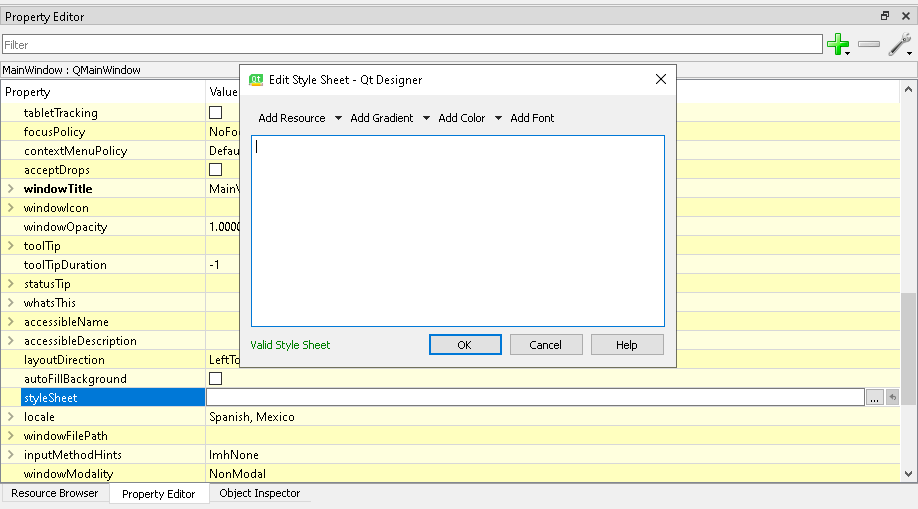
\includegraphics[scale=0.5]{imagenes/qtdesigner/stylesheets.PNG}
    \caption{Configurar el estilo desde QtDesigner}
    \label{fig:qt_stylesheet_image}
\end{figure}

Desde el c\'odigo la primera forma de hacerlo ser\'ia.

\begin{lstlisting}{language=Python}
    my_widget.setStyleSheet("background-color: black;")
\end{lstlisting}

Otra forma m\'as elegante y organizada ser'ia crear un archivo, supongamos \textbf{style.css} en donde
albergamos todo el estilo que vamos a usar con la correcta sint\'axis antedicha, entonces en el c\'odigo...

\begin{lstlisting}{language=Python}
    with open("styles.css") as f:
        my_widget.setStyleSheet(f.read())
\end{lstlisting}
